\originalchapter{神经网络与反向传播}\label{ch:nn}
\originalsection{非线性组合的必要性}
线性层叠加仍是线性层. 若 $h=A_1x+b_1$, $z=A_2h+b_2$, 则 $z=A_2A_1x+A_2b_1+b_2$. 因而单纯增加线性层数不会扩大可表示的函数族. 神经网络在层间插入非线性, 让不同输入激活不同的局部运算. 其价值是函数表示与可训练的组合结构, 不是“神经”一词本身.

\begin{definition}
两层多层感知机在列向量记号下写为 $a=W_1x+b_1$, $h=\phi(a)$, $z=W_2h+b_2$. $W_1\in\R^{r\times d}$, $W_2\in\R^{V\times r}$, 激活 $\phi$ 逐坐标作用. 标量激活可取 $\tanh a=(e^a-e^{-a})/(e^a+e^{-a})$ 或 $\operatorname{ReLU}(a)=\max(0,a)$.
\end{definition}
对二元输入的 XOR, 标签为 $y=x_1+x_2-2x_1x_2$. 若线性分类器能分开它, 对 $(1,0),(0,1)$ 要有 $w_1+b>0,w_2+b>0$, 而对 $(0,0),(1,1)$ 要有 $b<0,w_1+w_2+b<0$. 前两式相加给 $w_1+w_2+2b>0$, 后两式相加给同一量小于零, 矛盾. 非线性特征 $h_1=\operatorname{ReLU}(x_1-x_2)$, $h_2=\operatorname{ReLU}(x_2-x_1)$ 则使 $h_1+h_2$ 在 XOR 正例上为 1, 负例上为 0. 这构造了可分表示, 不依赖“网络足够大”的泛称.

\originalsection{单样本完整梯度}
令输出概率 $q=\softmax(z)$, 真实类别的 one-hot 向量为 $e_y$, 损失为 $\ell=-\log q_y$. 第 3 章已给出 $\delta_2=\nabla_z\ell=q-e_y$. 用第 4 章仿射映射的微分,
\begin{align*}
\nabla_{W_2}\ell&=\delta_2h^\top,&\nabla_{b_2}\ell&=\delta_2,\\
\nabla_h\ell&=W_2^\top\delta_2,&
\delta_1=\nabla_a\ell&=(W_2^\top\delta_2)\odot\phi'(a),\\
\nabla_{W_1}\ell&=\delta_1x^\top,&\nabla_{b_1}\ell&=\delta_1.
\end{align*}
$\odot$ 为逐坐标乘积. 对 $\tanh$, $\phi'(a)=1-\tanh^2a=1-h^2$. 先计算下游梯度再乘局部 Jacobian 的转置, 是反向传播的全套原则. 如果一个变量同时影响多条路径, 必须把路径贡献相加.

批量实现常把样本放在行上, 写 $H=\tanh(XW_1+b_1)$, $Z=HW_2+b_2$. 此时权重尺寸与列记号转置. 若 $D_2$ 已含平均损失的 $1/B$ 因子, 则 $\nabla W_2=H^\top D_2$, $\nabla b_2=\sum_i(D_2)_{i,:}$, $D_1=(D_2W_2^\top)\odot(1-H^2)$, $\nabla W_1=X^\top D_1$. 梯度中只能平均一次; 把所有层都再除以 $B$ 会错误缩小更新.

\begin{example}
一维隐层网络为 $a=wx$, $h=\tanh a$, $z=vh$, 损失为 $\ell=(z-y)^2/2$. 求对 $w,v$ 的导数.
\end{example}
\begin{solution}
输出处梯度为 $z-y$. 对 $v$ 得 $(z-y)h$; 对 $w$ 的路径依次经过 $v$, $1-h^2$ 和 $x$, 得 $(z-y)v(1-h^2)x$. 若先把网络完全展开为 $(v\tanh(wx)-y)^2/2$ 再求导, 会得到同样结果. 反向传播只是避免重复展开公共子表达式.
\end{solution}

\originalsection{批次轴与共享参数}\label{sec:tensor}
语言模型让每个样本含多个 token, 从二维表进入三维数组. 用 $B$ 表示文档数, $T$ 表示输入位置数, $D$ 表示特征数, $V_0$ 表示词表大小. 本节代码采用 Python 的零起下标: $b=0,\ldots,B-1$, $t=0,\ldots,T-1$, 词编号取 $0,\ldots,V_0-1$. 数组 \texttt{ids} 的形状是 $(B,T)$, 元素是整数编号; \texttt{E} 的形状是 $(V_0,D)$, \texttt{P} 是 $(T,D)$. 查表 \texttt{E[ids]} 把每个编号换成一行特征, 得到 $(B,T,D)$. 位置向量对每个文档共享, 因此
\[
x_{bti}=E_{\mathrm{ids}_{bt},i}+P_{ti}.
\]
代码 \texttt{x=E[ids]+P[:T]} 把 $P$ 的前面补一个长度为 1 的批次轴, 再沿 $B$ 复制使用. 这称为广播. 反向对共享的 $P_{ti}$ 收集所有文档的贡献: $(G_P)_{ti}=\sum_b(G_x)_{bti}$, 对应 \texttt{dx.sum(0)}. 偏置 $b_i$ 同时对所有文档和位置广播, 则 $G_{b_i}=\sum_{b,t}(G_y)_{bti}$, 对应 \texttt{dy.sum(axis=(0,1))}.

对于权重 $W\in\R^{D\times R}$, \texttt{x@W} 在每个 $(b,t)$ 的特征行上使用同一权重, 输出形状 $(B,T,R)$. 换成分量即 $y_{btr}=\sum_i x_{bti}W_{ir}$. 第 \ref{sec:frobenius} 节的系数比较现在多一个求和轴:
\[
(G_W)_{ir}=\sum_{b,t}x_{bti}(G_y)_{btr},\qquad G_x=G_yW^\top.
\]
\texttt{x.reshape(-1,D)} 把前两个轴合并成 $BT$ 行, 第 $bT+t$ 行就是原来的 $(b,t)$ 行, 保留最后的特征轴. 它没有求和、没有交换特征. 这样 \texttt{x.reshape(-1,D).T @ dy.reshape(-1,R)} 一次矩阵乘法完成上式的双重求和. 两个数组必须用相同的行顺序. 本项目的 \texttt{mm(x,y)} 就是这一操作. 平均交叉熵的 $1/(BT)$ 已进入 \texttt{dl}, 因而这里不再除以批次大小.

查表有相反方向的汇总: 若同一词在两个位置出现, 两条梯度路径属于同一参数行. 其数学定义为
\[
(G_E)_{vi}=\sum_{b,t:\,\mathrm{ids}_{bt}=v}(G_x)_{bti}.
\]
代码先创建零数组, 再用 \texttt{np.add.at(g['E'],ids,dx)} 按编号累加. 普通高级索引 \texttt{gE[ids] += dx} 可能先取出副本再写回, 重复编号的贡献不会可靠地逐次积累. 与位置向量求和一样, 本质是共享参数的所有路径都须相加.

\begin{exercise}
词表大小为 3, 特征维为 2. 两个位置的编号都是 1, 上游梯度分别为 $(2,-1)$ 和 $(3,4)$. 写出正确的词表梯度, 并实际比较高级索引与 \texttt{np.add.at}.
\end{exercise}
\begin{solution}
编号为 1 的行, 即数组的第二行, 应为 $(5,3)$, 其他行为零. 可运行如下代码; 本项目测试也检查这个共享路径不变量:
\begin{verbatim}
import numpy as np
ids = np.array([1, 1])
dx = np.array([[2., -1.], [3., 4.]])
good = np.zeros((3, 2)); bad = good.copy()
np.add.at(good, ids, dx)
bad[ids] += dx
print(good[1], bad[1])
\end{verbatim}
在本次 NumPy 环境中分别输出 \texttt{[5. 3.]} 与 \texttt{[3. 4.]}. 第二条语句不足以表达逐出现次数累加, 所以不应用它实现查表反向传播.
\end{solution}

\originalsection{计算图、初始化与残差}
对含共享子图的网络, 反向传播每条边只处理局部导数, 通常代价与前向同一数量级. 它需要保存前向中用于局部导数的激活, 因而训练内存通常大于单次推理. 自动微分框架实现的是运算图的求导规则, 不是自动判断数学目标是否适合任务. 错误的数据划分与损失定义仍会得到“正确计算”的梯度.

初始化全部相同会让多个隐单元接收相同输入、得到相同梯度, 对称性无法靠普通确定更新破除. 权重过大时 $\tanh$ 饱和, 导数接近零; 过小时信号可能逐层减弱. 一个粗略方差分析是假设输入分量独立、居中, 权重独立且方差为 $s^2$, 则 $a_j=\sum_{i=1}^d W_{ij}x_i$ 的方差约为 $ds^2\operatorname{Var}(x_i)$. 选择 $s^2$ 随 $1/d$ 缩放可控制信号尺度. 假设不严格满足时, 这个分析仍只是初始化的设计理由, 不是训练成功保证.

残差层 $h_{l+1}=h_l+F_l(h_l)$ 的 Jacobian 为 $I+J_{F_l}$. 它提供一条直接的恒等路径, 但多层乘积依然可能爆炸或衰减, 所以不能声称残差必然消除梯度问题. 层归一化对每个 token 的特征计算均值 $\mu$ 和方差 $s^2$, 再输出 \mbox{$\gamma\odot(h-\mu)/\sqrt{s^2+\epsilon}+\beta$}. $\gamma,\beta$ 是可训练向量. 方差中的 $\epsilon$ 防止退化除零. 首版手写小模型省略归一化, 为减少实现与梯度检查负担; 现代标准 Transformer 通常包含它或 RMSNorm.

\originalsection{实验与练习}
实验 \texttt{mlp} 使用 8 个 $\tanh$ 隐单元, 两个 softmax 输出, 对 XOR 的全部四点训练 4,000 次, 步长为 0.1. 初始化与训练均固定种子, 所有参数组都有有限差分抽样. 它检验“非线性表示能拟合 XOR”与“反向传播实现相符”, 没有独立测试样本, 因而不报告自然数据泛化能力. 损失曲线来自实际执行, 在图 \ref{fig:mlp} 中显示.
\begin{figure}[ht]
\centering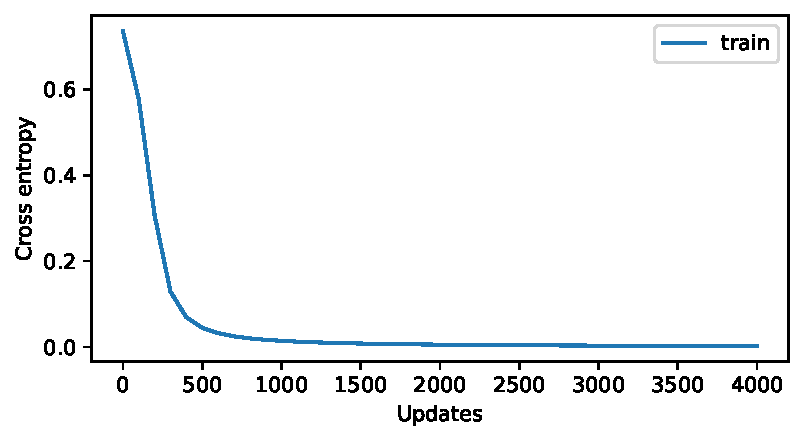
\includegraphics[width=.66\textwidth]{generated/mlp.pdf}
\caption{XOR 平均交叉熵随更新步数变化. 单个固定种子, 横轴为实际更新次数.}\label{fig:mlp}
\end{figure}

\begin{exercise}
若同一矩阵 $W$ 在两条支路分别产生 $Wx$ 和 $Wu$, 对应下游梯度分别为 $a,b$, 求总梯度.
\end{exercise}
\begin{solution}
两条路径微分相加为 $a^\top dW\,x+b^\top dW\,u$, 所以总梯度为 $ax^\top+bu^\top$. 共享参数的梯度不能由其中一条支路覆盖另一条.
\end{solution}
\begin{exercise}
若两层网络没有非线性, 为什么仍可能与直接优化一个线性矩阵有不同训练行为?
\end{exercise}
\begin{solution}
可表示函数仍是线性, 但参数化为 $W_2W_1$ 后目标对这两组因子一般非凸, 梯度分别依赖另一因子. 参数空间的尺度对称性、隐式偏置与优化轨迹都可能不同. 函数族相同不意味着优化问题相同.
\end{solution}
\label{ch:end:06}
